\chapter{Another chapter}\label{ch:results}

\section{Ground State Degeneracy}
In this chapter results of simulations on the dipolar kagome lattice are presented. EFM simulations reveal a many-fold degenerate ground state allowing zero-temperature states comprising a six-sublattice structure; three of the sublattices contain spins that are the negatives of the spins on the remaining three sublattices. The spins alternate in direction along the [1,1,1] direction.

\begin{figure}
	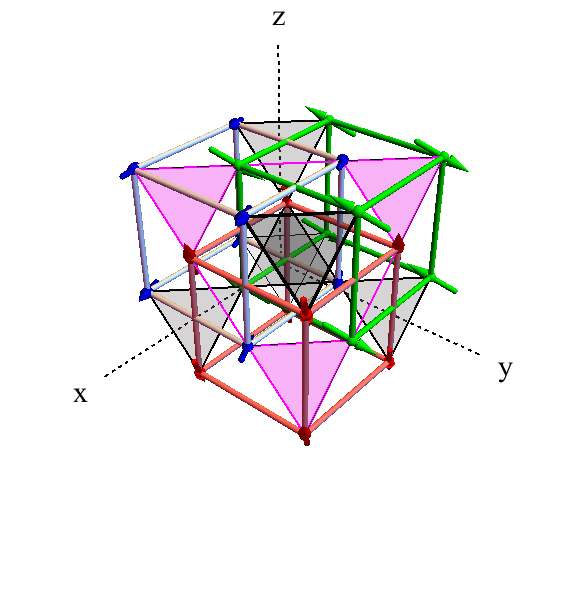
\includegraphics[width=\linewidth]{img/3dfcc.png}
	\caption{A view down the <1,1,1> axis of a 3D FCC lattice with six sub-lattice spin vectors.}
	\label{fig:3dfcc}
\end{figure}

\clearpage
Every ground state configuration obtained through the EFM simulation is characterized by the following set of equations:
\begin{equation}
\label{eqn:rel_a}
\alpha = \sin{\theta} \cos{\phi}
\end{equation}
\begin{equation}
\label{eqn:rel_b}
\beta = \sin{\theta} \sin{\phi}
\end{equation}
\begin{equation}
\label{eqn:rel_c}
\chi = \cos{\theta}
\end{equation}
\begin{equation}
\label{eqn:rel_d}
\delta = (2a^2-1)/2c
\end{equation}
\begin{equation}
\label{eqn:rel_e}
\epsilon = \sqrt(1-a^2-d^2)
\end{equation}

This set of equations acts as elementary building blocks for the components of the spin vectors that exist in the dipolar kagome ground state. There are two parameters that dictate the resulting ground state: $\theta$ and $\phi$, which are polar angles of the spin "A". Spin A is arbitrarily chosen. The spin vectors themselves may be constructed as follows:

$$\overrightarrow{a} = (\alpha, \beta, \chi)$$
$$\overrightarrow{b} = (\delta, \epsilon, -\alpha)$$
$$\overrightarrow{c} = (-\epsilon, -\chi-\delta, \beta)$$
$$\overrightarrow{d} =-\overrightarrow{a}$$
$$\overrightarrow{e} =-\overrightarrow{b}$$
$$\overrightarrow{f} =-\overrightarrow{c}$$

\clearpage

\begin{figure}
	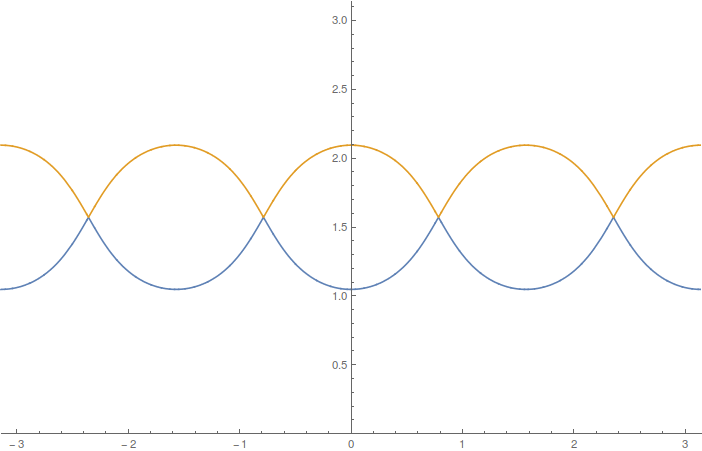
\includegraphics[width=\linewidth]{img/degeneracyplanefull.png}
	\caption{A plane that contains points that allow the construction of valid ground states.}
	\label{fig:degenplanefull}
\end{figure}


Any theta and phi pair chosen from the plane in figure \ref{fig:degenplanefull} will give rise to a valid ground state of the same energy with the exception of those pairs of theta and phi that lie within the bound region of the graph. Within the bound region of the graph, e = √(1–a²–d²) ∈ ℂ. At each node of each bound area, d = (2a²–1)/2c → ±0/0.

\begin{figure}
	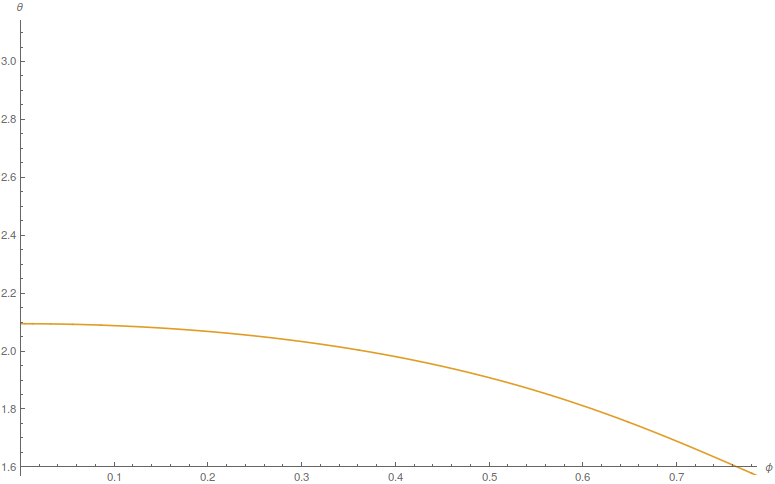
\includegraphics[width=\linewidth]{img/degeneracyplane.png}
	\caption{One section of the original degeneracy plane that is equivalent to all other sections of the plane due to symmetry operations.}
	\label{fig:degenplane}
\end{figure}

It is possible to reduce the size of this graph to 1/16 the size by showing that a state in each portion of the graph is relatable to an analogous state in the other portions of the graph via symmetry operations.
\clearpage

\subsection{Visualization of the Ground State}

By generating the spin vectors described by equations \ref{eqn:rel_a},\ref{eqn:rel_b},\ref{eqn:rel_c},\ref{eqn:rel_d}, and \ref{eqn:rel_e}, spin configurations ranging from planar to non-planar states can be obtained. An example of a non-planar state is shown in figure \ref{fig:sampgs}.

\begin{figure}[ht]
	%TODO Change this image with a better one
	\centering
	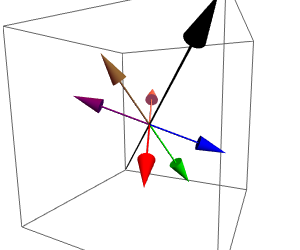
\includegraphics[scale=0.9]{img/samplegs.png}
	\caption{The six sublattice spins conjoined at their ends for clarity and illustration. The vector denoting <1,1,1> axis of symmetry is illustrated in black}
	\label{fig:sampgs}
\end{figure}

To gain insight into what choices of $\theta$ and $\phi$ pairs give rise to particular states, consider the contour plot in fig. \ref{fig:gsvol}. The contour plot illustrates the volume of a parallelopiped formed by the a, b, and c spin vectors corresponding to a particular $\theta$ and $\phi$ chosen from fig. \ref{fig:degenplane}. It is from this illustration that one can obtain an understanding of what choices of $\theta$ and $\phi$ result in planar states or non-planar states.


\begin{figure}[ht]
	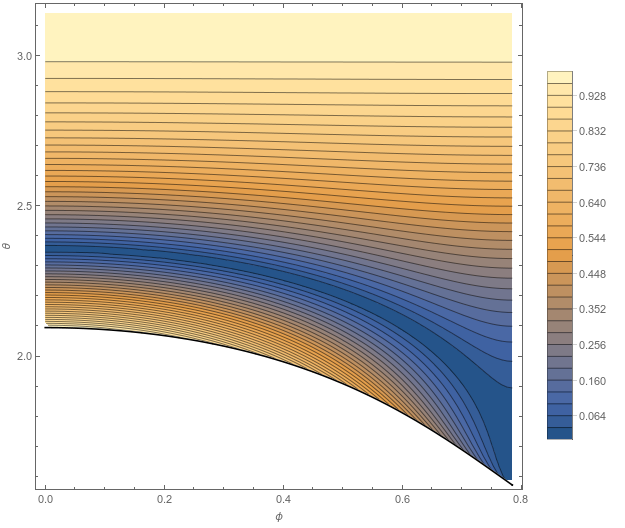
\includegraphics[width=\linewidth]{img/groundstatevol.png}
	\caption{A contour plot of volume of a parallelopiped formed by a spin configuration with respect to $\theta$ and $\phi$ }
	\label{fig:gsvol}
\end{figure}
\clearpage

\begin{figure}[ht]
\centering
	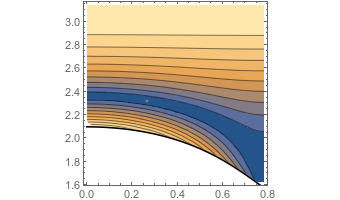
\includegraphics[scale=1.3]{img/th2-3108_phi0-27_plane.png}
	\caption{A contour plot of volume of a parallelepiped with respect to theta and phi. The point corresponding to theta=2.3108 and phi=0.27 is highlighted in green.}
	\label{fig:volplane_ex}
\end{figure}

As an example, the point corresponding to a planar state located at the point $\theta$=2.3108 and $\phi$=0.27 was chosen, as shown in fig. \ref{fig:volplane_ex}.

\begin{figure}
  \label{fig:volplaneex_vecs}
  \begin{minipage}[b]{0.5\linewidth}
    \centering
    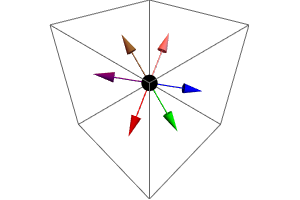
\includegraphics[width=.8\linewidth]{img/th2-3108_phi0-27_view1.png} 
    \caption{View 1} 
    \vspace{4ex}
  \end{minipage}%%
  \begin{minipage}[b]{0.5\linewidth}
    \centering
    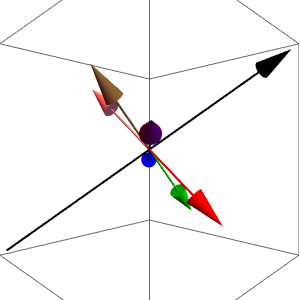
\includegraphics[width=.5\linewidth]{img/th2-3108_phi0-27_view2.png} 
    \caption{View 2} 
    \vspace{4ex}
  \end{minipage} 
  \begin{minipage}[b]{0.5\linewidth}
    \centering
    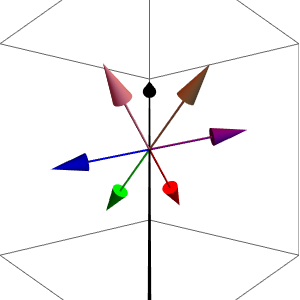
\includegraphics[width=.5\linewidth]{img/th2-3108_phi0-27_view3.png} 
    \caption{View 3} 
    \vspace{4ex}
  \end{minipage}%% 
  \begin{minipage}[b]{0.5\linewidth}
    \centering
    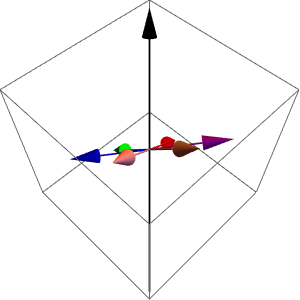
\includegraphics[width=.5\linewidth]{img/th2-3108_phi0-27_view4.png} 
    \caption{View 4} 
    \vspace{4ex}
  \end{minipage} 
  \caption{Four different perspectives of the same spin configuration corresponding to theta=2.3108 and phi=0.27}
\end{figure}

Using equations \eqref{eqn:rel_a},\eqref{eqn:rel_b},\eqref{eqn:rel_c},\eqref{eqn:rel_d}, and \eqref{eqn:rel_e}, the vectors were conjoined as shown in fig. \ref{fig:volplaneex_vecs}.

\clearpage
\subsection{Planar Ground States}

The thin strip of blue that cuts into the contour plot just above the complex region consists of the set of points that give rise to parallelopipeds with the smallest volume. This corresponds to spin configurations that are planar. Elsewhere in the plane, the spin configurations are non-planar. The strip of points that give rise to planar states are described by the following polar equations:

\begin{equation}
\phi = \frac{\pi}{4}\cos{\gamma} 
\end{equation}
\begin{equation}
\theta = \frac{\pi}{4}(\sin{\gamma}+2)
\end{equation}

The spin configurations that are planar can therefore be described in terms of one parameter, $\gamma$, the polar equations which determine $\theta$ and $\phi$, and the original set of equations.  

\begin{figure}[h]
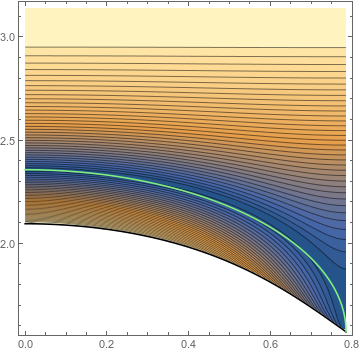
\includegraphics[width=.5\linewidth]{img/groundstatevol_withplanarborder.png} 
    \caption{Contour plot of parallelepiped volume with the perimeter of a circle shown in green.} 
\end{figure}
\clearpage
\section{3D Dipolar Kagome Finite T EFM Results}


\section{3D Dipolar Kagome Magnetic Field EFM Results}

In this section results on application of an external magnetic field on the dipolar kagome lattice are presented. EFM simulations revealed how a sufficiently large external magnetic field caused the spin configuration to transition from a non-planar state to a planar state. Following this transition, the spins underwent a linear change in orientation with respect to magnetic field magnitude by reorienting in the direction of the magnetic field. Following degaussing, the spins unaligned with the magnetic field and form a planar state at zero magnetic field magnitude, regardless of whether the state was initially non-planar. In essence, when degaussing with a sufficiently high peak magnetic field magnitude, any minimum-energy state was transformed into a planar state. Finally, with sufficiently high magnetic field magnitude, the lattice became saturated and the rate at which the spins reoriented themselves along the direction of the magnetic field was reduced. 

\subsection{Magnetic Phases}

The magnetization as a function of magnetic field magnitude of the 3D kagome lattice had several distinct phases of change. In figure \ref{fig:magphase}, the magnetization lingered close to zero at low magnetic field magnitude. A sudden change in magnetization occured for all non-planar states, after which a planar state was formed. A linear change in magnetization was observed after this critical field magnitude, until the lattice became saturated and the magnetization nearly plateaued.

\begin{figure}
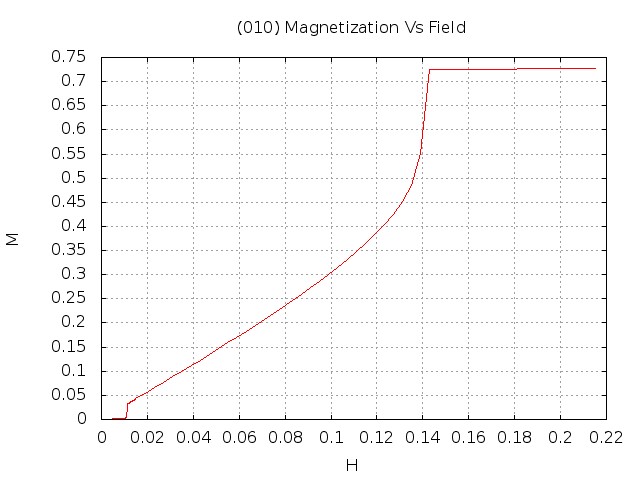
\includegraphics[scale=0.7]{img/magneticphases.png}
\caption{A curve of magnetization with respect to changing magnetic field magnitude of a magnetic field oriented along the y-axis.}
\label{fig:magphase}
\end{figure}

\subsection{Degaussing Along a Cube Axis}

\subsubsection{(001) Increasing Field}
%theta=0.206275 phi=3.11867 for starting state
\paragraph
\large
The 6 spins begin to transition to the planar state at H=0.0105 and achieves the planar state at H=0.0121.
The pink and brown spins swap positions, as do the blue and purple spins, as the field is increased beyond the planar state. 
The spins gradually align with the 001 field direction, until approximately at 0.14 the lattice becomes saturated and
the red and green and spins become parallel to the field direction. 
\begin{figure}[ht]
\centering
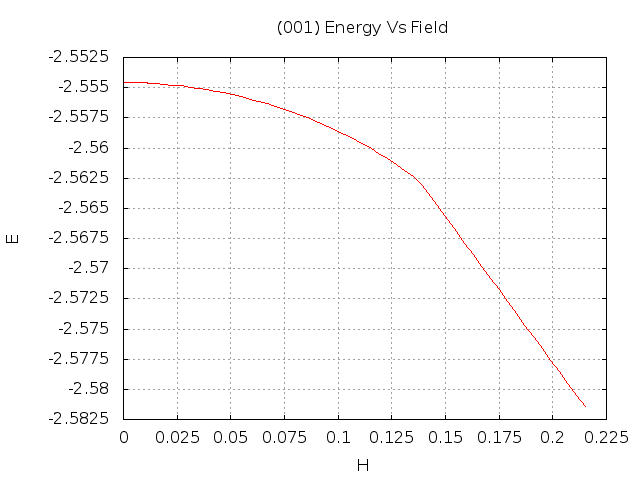
\includegraphics[scale=0.3]{25june16/HVariedData/Increasing/001Einc.png}
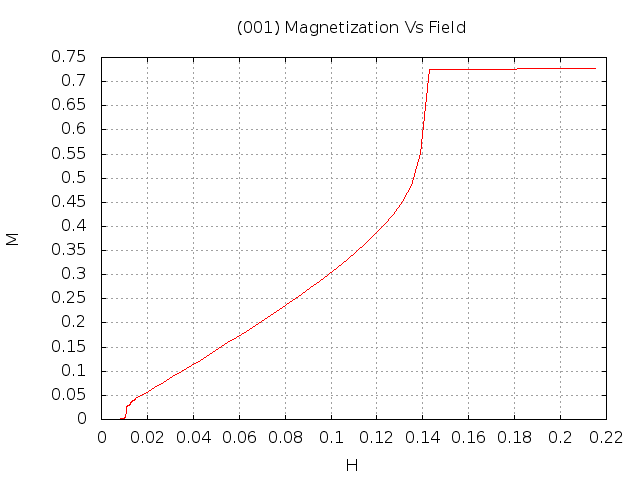
\includegraphics[scale=0.3]{25june16/HVariedData/Increasing/001Minc.png}
\end{figure}
\begin{figure}[ht]
\centering
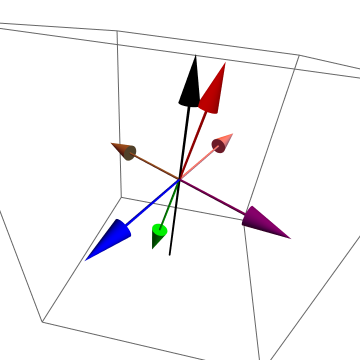
\includegraphics[scale=0.3]{25june16/HVariedData/Pictures/001Inc1.png}
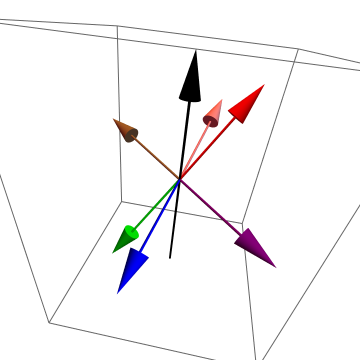
\includegraphics[scale=0.3]{25june16/HVariedData/Pictures/001Inc106.png}
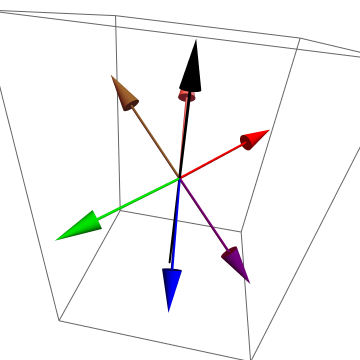
\includegraphics[scale=0.3]{25june16/HVariedData/Pictures/001Inc122.png}
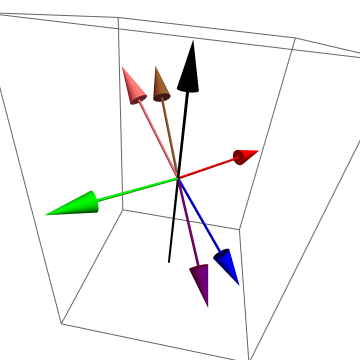
\includegraphics[scale=0.3]{25june16/HVariedData/Pictures/001Inc151.png}
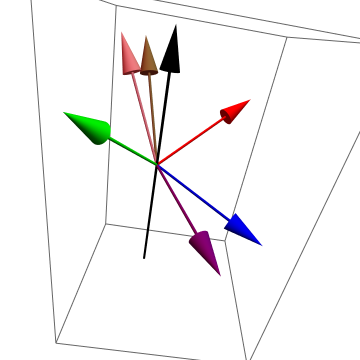
\includegraphics[scale=0.3]{25june16/HVariedData/Pictures/001Inc30S.png}
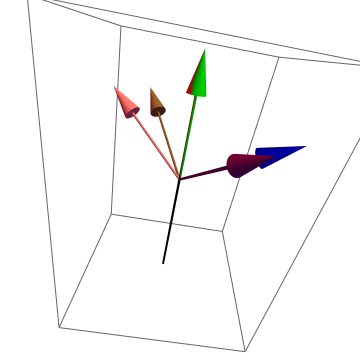
\includegraphics[scale=0.3]{25june16/HVariedData/Pictures/001Inc35S.png}
\caption{Snap shots of the 6 characteristic spins at H=0, 0.0105, 0.0121, 0.0150, 0.131, 0.151. The black arrow
indicates the direction of the field. In the dot product graph, AB dot product goes to zero once the lattice 
is saturated. This agrees with A and B (red and green) lining up in the above snapshots.}
\end{figure}
\clearpage

\subsubsection{(001) Decreasing Field}
%theta=0.206275 phi=3.11867 for starting state. Even for decreasing field??
\paragraph
\large
The lattice leaves the saturated state at a field lower than what was required to induce it while increasing the field.
This transition from saturation occurs at approximately H=0.13, compared to the transition to saturation at H=0.14 when increasing the field. %Description here
The spins gradually unalign and rest in a planar state at zero field, and is characterized by the groundstate angles theta=89.9 degrees and phi=44.94 degrees.
\begin{figure}[ht]
\centering
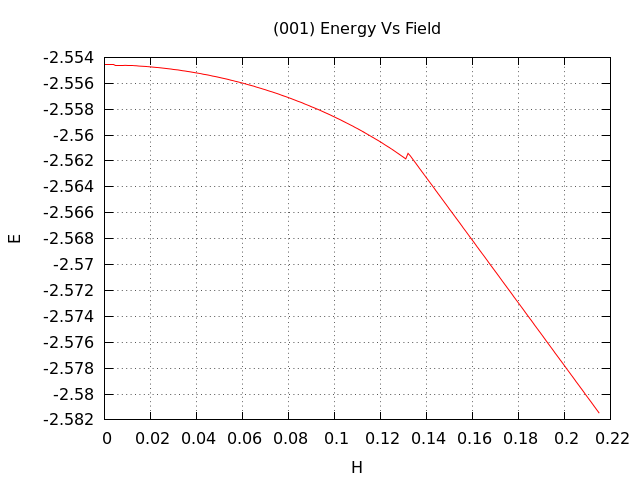
\includegraphics[scale=0.3]{25june16/HVariedData/Decreasing/001Edec.png}
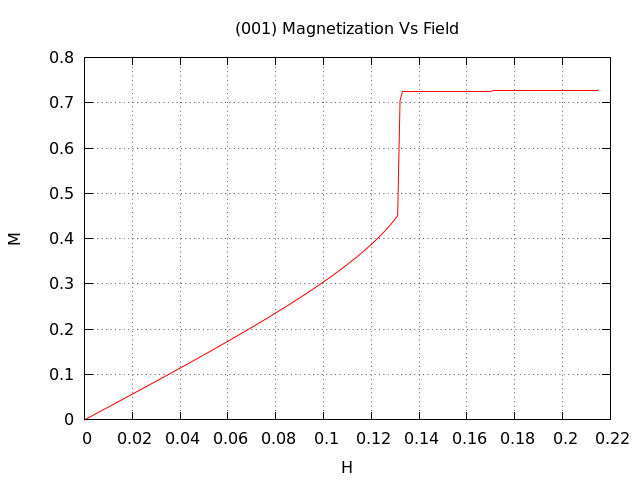
\includegraphics[scale=0.3]{25june16/HVariedData/Decreasing/001Mdec.png}
\end{figure}
\begin{figure}[ht]
\centering
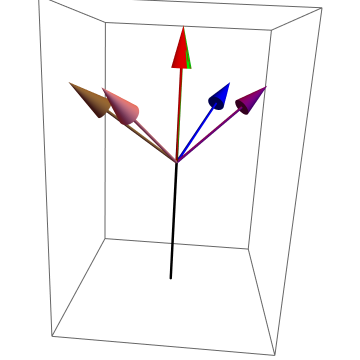
\includegraphics[scale=0.37]{25june16/HVariedData/Pictures/001Dec1.png}
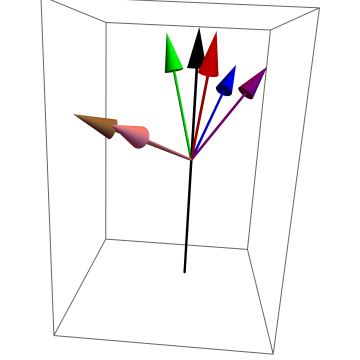
\includegraphics[scale=0.37]{25june16/HVariedData/Pictures/001Dec84.png}
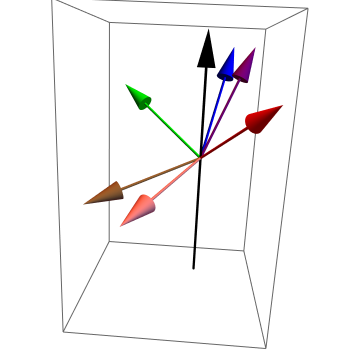
\includegraphics[scale=0.37]{25june16/HVariedData/Pictures/001Dec86.png}
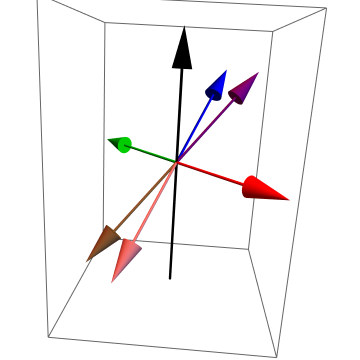
\includegraphics[scale=0.37]{25june16/HVariedData/Pictures/001Dec216.png}
\caption{Snapshots at H=0.215, 0.132, 0.130, 0}
\end{figure}

\begin{figure}[ht]
\centering
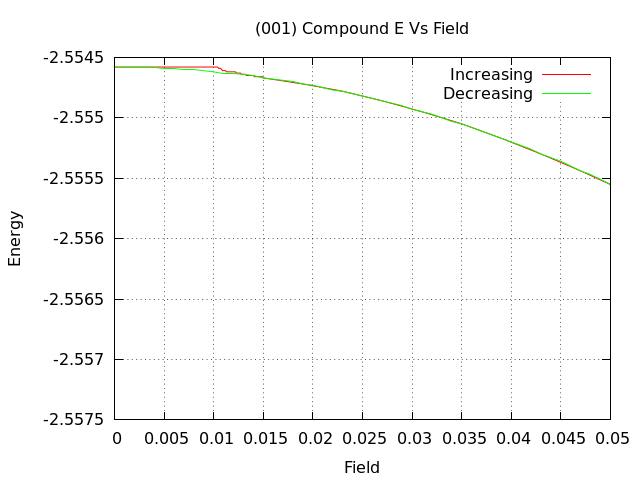
\includegraphics[scale=0.5]{25june16/HVariedData/compoundEM/001Ecompound.png}
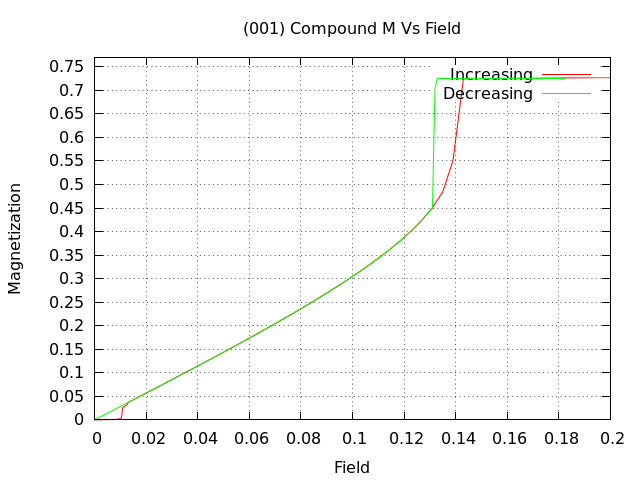
\includegraphics[scale=0.5]{25june16/HVariedData/compoundEM/001Mcompound.png}
\caption{Composite graphs of energy and magnetization for both decreasing and increasing field magnitude. Note the
different scales for the energy and magnetization graph. This is because plotting energy vs field on a graph
which has an xrange of 0.2 reduces the ability to see any difference in the energy curves. This was done for all 
composite graphs.}
\end{figure}
\clearpage
\subsection{Degaussing Along a Cube Face}
\subsubsection{(011) Increasing Field}
\paragraph
\large
The lattice begins to transition at approximately 0.007. At 0.0074 the planar state is achieved. At 0.0093, the 
pink and red spins swap position, and the blue and green spins swap position. As the field is increased further to 0.0115,
the green and brown spins begin to swap positions. At 0.143, this is achieved. Once saturated, no spins are parallel
with the field direction.%Description here

\begin{figure}[ht]
\centering
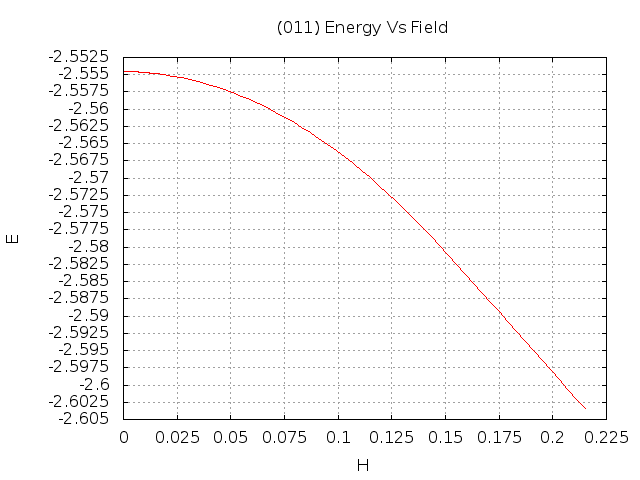
\includegraphics[scale=0.3]{25june16/HVariedData/Increasing/011Einc.png}
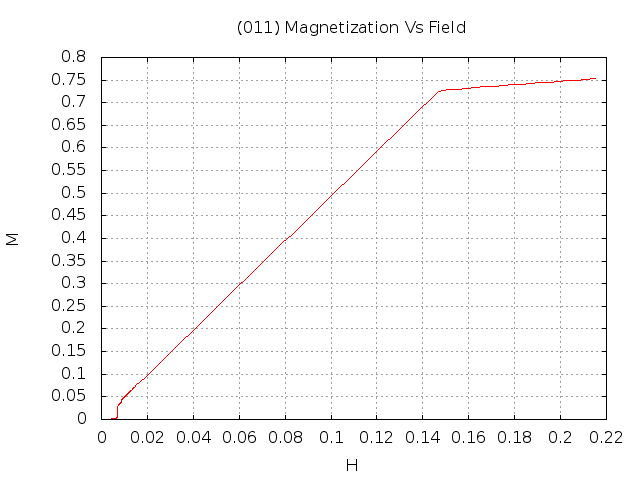
\includegraphics[scale=0.3]{25june16/HVariedData/Increasing/011Minc.png}
\end{figure}
\begin{figure}[ht]
\centering
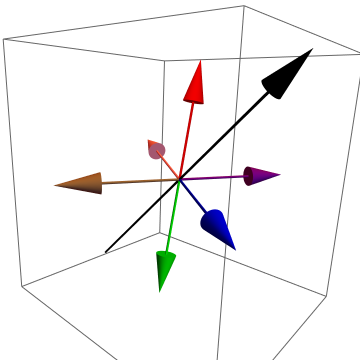
\includegraphics[scale=0.3]{25june16/HVariedData/Pictures/011Inc1.png}
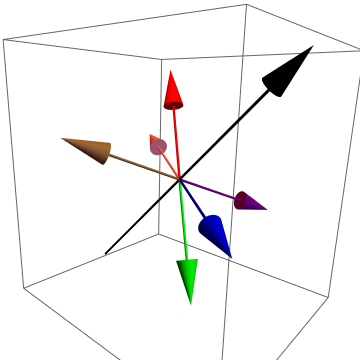
\includegraphics[scale=0.3]{25june16/HVariedData/Pictures/011Inc67.png}
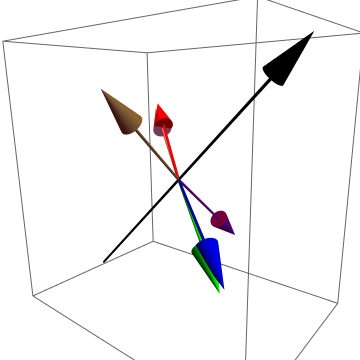
\includegraphics[scale=0.3]{25june16/HVariedData/Pictures/011Inc82.png}
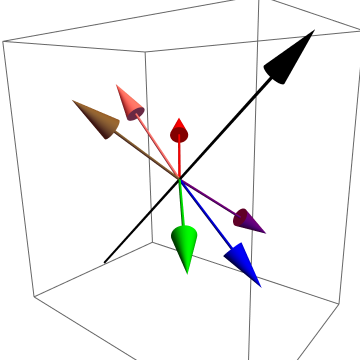
\includegraphics[scale=0.3]{25june16/HVariedData/Pictures/011Inc94.png}
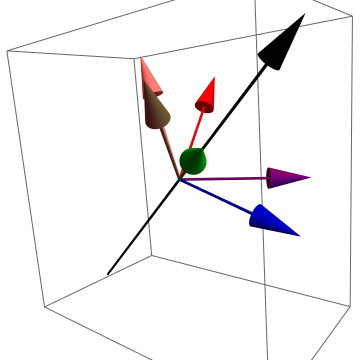
\includegraphics[scale=0.3]{25june16/HVariedData/Pictures/011Inc26S.png}
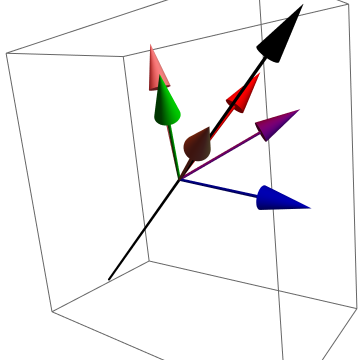
\includegraphics[scale=0.3]{25june16/HVariedData/Pictures/011Inc39S.png}
\caption{Snapshots at H=0, 0.0066, 0.0082, 0.0094, 0.115, 0.167}
\end{figure}

\clearpage

\subsubsection{(011) Decreasing Field}
\paragraph
\large
As the field is decreased to 0.134, the brown and green spins swap positions again. All 6 spins gradually unalign
with the field until they reach a zero field planar state characterized by angles theta=69.33 degrees and phi=-139.133 degrees.%Description here

\begin{figure}[ht]
\centering
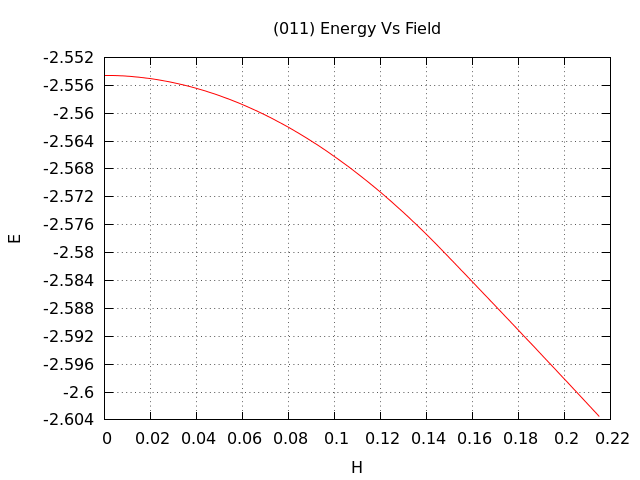
\includegraphics[scale=0.3]{25june16/HVariedData/Decreasing/011Edec.png}
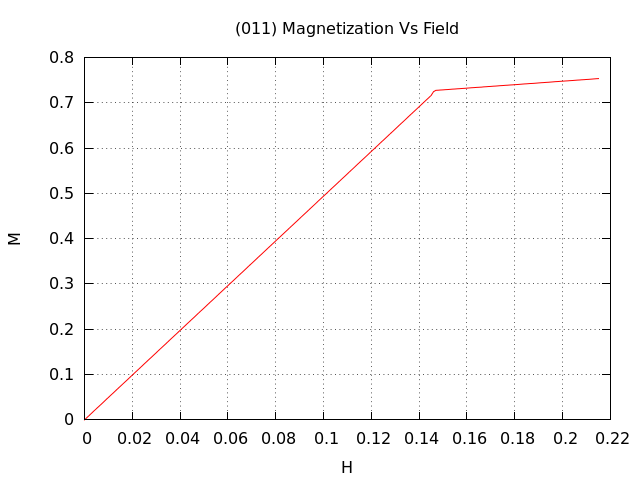
\includegraphics[scale=0.3]{25june16/HVariedData/Decreasing/011Mdec.png}
\end{figure}
\begin{figure}[ht]
\centering
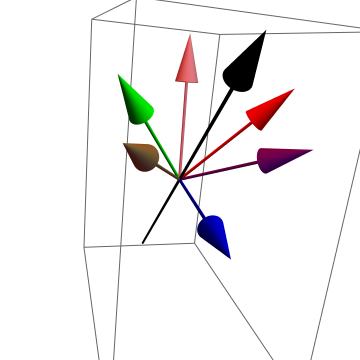
\includegraphics[scale=0.37]{25june16/HVariedData/Pictures/011Dec1.png}
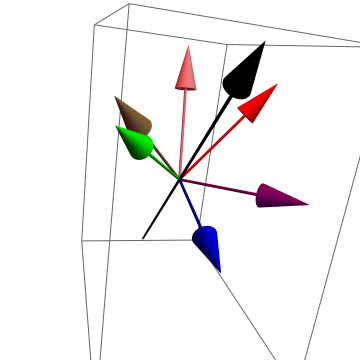
\includegraphics[scale=0.37]{25june16/HVariedData/Pictures/011Dec82.png}
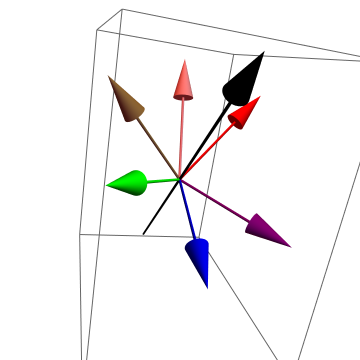
\includegraphics[scale=0.37]{25june16/HVariedData/Pictures/011Dec122.png}
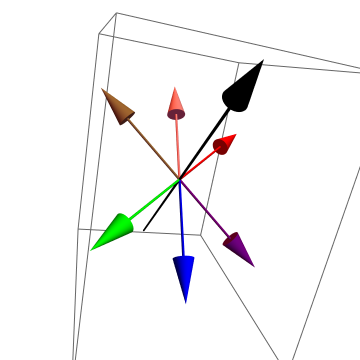
\includegraphics[scale=0.37]{25june16/HVariedData/Pictures/011Dec216.png}
\caption{Snapshots at H=0.215, 0.134, 0.094, 0}
\end{figure}

\subsection{Saturation of the Lattice}
Using the same groundstate as used in all simulations, 7 simulations were run with differing field directions. The 
field was increased up until saturating the lattice. 001 and 010 both have identical magnetization curves, as do
011 and 101. However, 100 differs from 001 and 010, and 110 differs from 011 and 101, which is unexpected. When using
the 111 field direction, saturation occurs at a field that is higher than the saturation fields of any other simulations. 
\begin{figure}[ht]
 \centering
 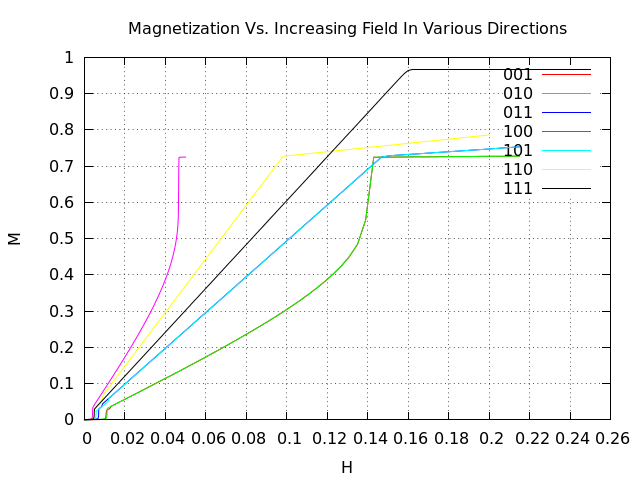
\includegraphics[scale=0.6]{25june16/HVariedData/Increasing/IncreasingField.png}
 \caption{Magnetization curves starting with the same ground state and subjected to fields of various directions}
\end{figure}
\clearpage

\subsection{Reduction of the Ground State Degeneracy via Application of an External Magnetic Field}

\begin{figure}[ht]
 \centering
 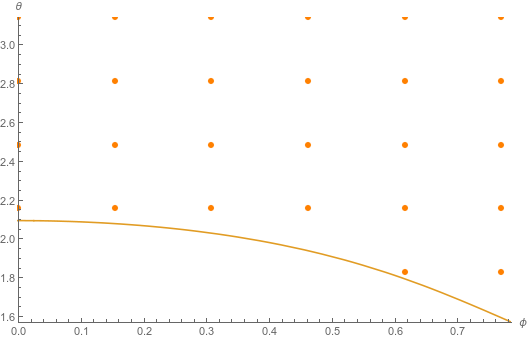
\includegraphics[scale=0.6]{img/predegaussed.png}
 \caption{The ground state plane with an array of points selected to generate the starting states for independent degaussing simulations.}
\end{figure}

\begin{figure}[ht]
 \centering
 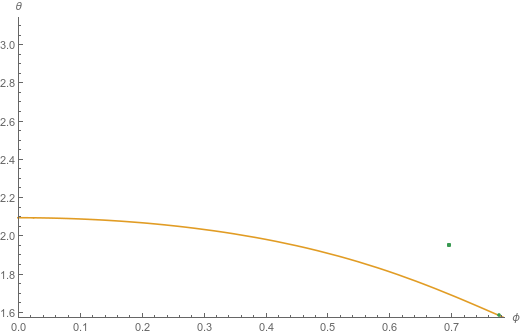
\includegraphics[scale=0.6]{img/postdegaussed.png}
 \caption{The final states following degaussing. All states are within the planar region of the plane.}
\end{figure}